\chapter{Réalisation et tests}

\section{Introduction}
Cette phase vise à concrétiser la conception sous forme d'une application fonctionnelle, suivie d'une série de tests de validation. Les maquettes d'interfaces ont été conçues à l'aide de l'outil Draw.io afin de prévisualiser et valider l'ergonomie avant le développement.

\section{Réalisation}
\subsection{Environnement de développement}
Cette solution s'appuie sur une stack technologique moderne, répartie entre frontend et backend.

Le frontend est réalisé avec :
\begin{itemize}
  \item \textbf{React} : pour la création des composants d'interface utilisateur ;
  \item \textbf{Vite} : pour un environnement de développement rapide et optimisé ;
  \item \textbf{TypeScript} : pour la robustesse du typage statique ;
  \item \textbf{Tailwind CSS} : pour une interface moderne  ;
  \item \textbf{Axios} : pour la communication HTTP client-serveur.
\end{itemize}

Le backend repose sur une architecture moderne et robuste composée de :
\begin{itemize}
  \item \textbf{Node.js} et \textbf{Express.js} : pour la gestion de la logique métier et la conception d'une API REST ;
  \item \textbf{Prisma} : comme ORM (Object-Relational Mapping) pour l'abstraction et la gestion de la base de données ;
  \item \textbf{PostgreSQL} : comme système de gestion de base de données relationnelle ;
  \item \textbf{Uploadthing} : pour la gestion et l'hébergement sécurisé des fichiers ;
  \item \textbf{JWT (JSON Web Tokens)} : pour l'authentification et l'autorisation sécurisées des utilisateurs.
  \item \textbf{Pino} : pour le logging et la gestion des erreurs.
\end{itemize}

Pour le déploiement de l'application, nous avons choisi d'utiliser le service \textbf{Railway}  comme service de gestion de conteneurs et de mise en production.
Le code source est géré via Git, un système de contrôle de version distribué, et hébergé sur GitHub afin de faciliter la collaboration et le suivi des modifications.
\subsection{Outils logiciels utilisés}

Cette section présente les principaux outils logiciels ayant été utilisés dans le cadre du développement du projet.

\begin{table}[H]
  \centering
  \begin{tabular}{| c | m{8cm} |}
    \hline
    \textbf{Outil} & \textbf{Utilisation principale} \\ 
    \hline

    \begin{minipage}{.4\linewidth}
        \centering
        \includegraphics[width=2.5cm]{images/logos/VsCode.png}
    \end{minipage} 
    & \textbf{Visual Studio Code} : Éditeur de code source léger et puissant utilisé pour le développement frontend (React, TypeScript) et backend (Node.js, Express). Il offre une large collection d’extensions, un terminal intégré, et une interface personnalisable. \\
    \hline

    \begin{minipage}{.4\linewidth}
        \centering
        
\includegraphics[width=2.5cm]{images/logos/Github.png}
    \end{minipage} 
    & \textbf{GitHub} : Plateforme de gestion de version basée sur Git. Utilisée pour héberger le code, collaborer entre membres du binôme, suivre les modifications, gérer les branches et assurer la traçabilité du développement. \\
    \hline

    \begin{minipage}{.4\linewidth}
        \centering
        
\includegraphics[height=2.5cm]{images/logos/overleaf.png}
    \end{minipage} 
    & \textbf{Overleaf} : Éditeur en ligne collaboratif basé sur LaTeX. Utilisé pour la rédaction du rapport de projet, la gestion des figures, tableaux, références bibliographiques, et pour assurer un format académique rigoureux. \\
    \hline

    \begin{minipage}{.4\linewidth}
        \centering
        
\includegraphics[width=2.2cm]{images/logos/Draw.io.png}
    \end{minipage} 
    & \textbf{Draw.io} : Outil de création de diagrammes UML (use case, séquence, classes). Utilisé pour modéliser les interactions et la structure du système. \\
    \hline

    \begin{minipage}{.4\linewidth}
        \centering
        
\includegraphics[width=2.2cm]{images/logos/React.png}
    \end{minipage} 
    & \textbf{React.js} : Bibliothèque JavaScript utilisée pour construire des interfaces utilisateur dynamiques et modulaires sous forme de composants. \\
    \hline

    \begin{minipage}{.4\linewidth}
        \centering
        
\includegraphics[width=2.2cm]{images/logos/Vite.js.png}
    \end{minipage} 
    & \textbf{Vite} : Serveur de développement moderne permettant un rechargement rapide des composants React et une compilation optimisée du projet. \\
    \hline

    \begin{minipage}{.4\linewidth}
        \centering
        
\includegraphics[width=2.2cm]{images/logos/TailwindCSS.png}
    \end{minipage} 
    & \textbf{Tailwind CSS} : Framework CSS utilitaire permettant une conception rapide et responsive des interfaces sans écrire de CSS personnalisé. \\
    \hline

    \begin{minipage}{.4\linewidth}
        \centering
        
\includegraphics[width=2.2cm]{images/logos/Prisma.png}
    \end{minipage} 
    & \textbf{Prisma} : ORM moderne pour Node.js. Utilisé pour interagir avec la base de données PostgreSQL à l’aide d’un modèle de données typé et sécurisé. \\
    \hline
\end{tabular}
\end{table}


\begin{table}[H]
  \centering
  \begin{tabular}{| c | m{8cm} |}
    \hline
        \begin{minipage}{.4\linewidth}
        \centering
        \includegraphics[width=2.2cm]{images/logos/PostgreSql.png}
    \end{minipage} 
    & \textbf{PostgreSQL} : Système de gestion de base de données relationnelle robuste, utilisé pour stocker et gérer les données de l’application (demandes, utilisateurs, rôles, etc.). \\
    \hline

    \begin{minipage}{.4\linewidth}
        \centering
        
\includegraphics[width=2.2cm]{images/logos/NodeJS.png}
    \end{minipage} 
    & \textbf{Node.js} et \textbf{Express.js} : Technologies backend utilisées pour gérer les routes, la logique métier, les vérifications de rôles et les appels à la base de données via API REST. \\
    \hline

    \begin{minipage}{.4\linewidth}
        \centering
        
\includegraphics[width=2.2cm]{images/logos/Uploadthing.png}
    \end{minipage} 
    & \textbf{Uploadthing} : Service de gestion de fichiers permettant le téléchargement, la prévisualisation et le stockage sécurisé des photos de profil et des pièces jointes. \\
    \hline

    \begin{minipage}{.4\linewidth}
        \centering
        
\includegraphics[width=2.2cm]{images/logos/JWT.png}
    \end{minipage} 
    & \textbf{JWT (JSON Web Token)} : Utilisé pour l’authentification sécurisée et la gestion des sessions utilisateur via des jetons cryptés. \\
    \hline

    \begin{minipage}{.4\linewidth}
        \centering
        
\includegraphics[width=2.2cm]{images/logos/axios.png}
    \end{minipage} 
    & \textbf{Axios} : Bibliothèque JavaScript utilisée pour envoyer des requêtes HTTP du frontend vers le backend, facilitant la communication entre les couches de l’application. \\
    \hline
  \end{tabular}
  \caption{Outils logiciels utilisés dans le développement de la plateforme IReSCoMath}
  \label{tab:outils_irescomath}
\end{table}

\subsection{Architecture générale}
L'utilisateur accède à l'interface et effectue des actions. Le frontend envoie alors, à l’aide de la bibliothèque Axios, une requête HTTP au backend, qui effectue les opérations nécessaires et renvoie une réponse.

Cette réponse est ensuite traitée par Axios et affichée à l’utilisateur, ou bien elle est utilisée pour mettre à jour l’interface. Le backend, développé avec le framework Express, reçoit les requêtes HTTP, les traite selon l'organisation de ses routes, accède aux données via Prisma et la base de données PostgreSQL, puis envoie une réponse au format JSON.

Dans le cas du téléversement de fichiers, le backend envoie une requête contenant le fichier à la plateforme UploadThing, qui retourne ensuite l’URL du fichier stocké.

Le schéma suivant présente l'architecture générale de l’application, en mettant en évidence les principales interactions entre ses composants :

\begin{figure}[H]
  \centering
  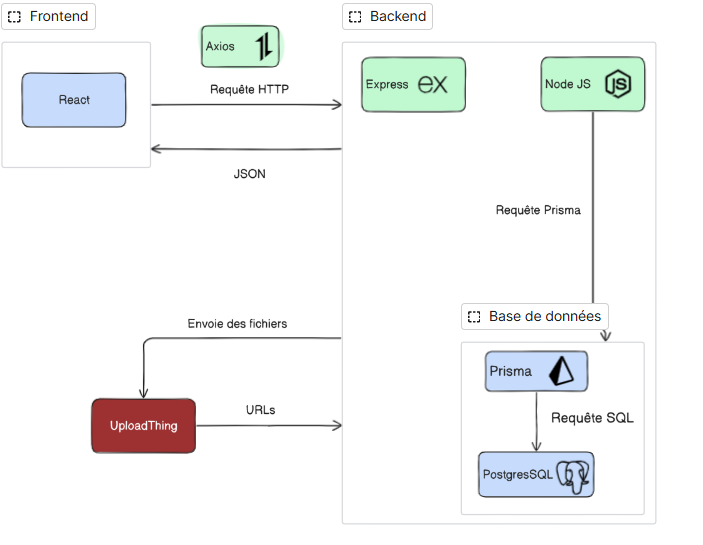
\includegraphics[width=0.7\textwidth]{images/architecture.png}
  \caption{Architecture générale de l'application}
  \label{fig:architecture_générale}
\end{figure}

\subsection{Environnement matériel}
Le projet a été développé sur deux ordinateurs portables appartenant aux membres du binôme.Chaque membre du binôme a travaillé sur un ordinateur portable sous Windows. Ces machines disposent d’une configuration matérielle suffisante pour assurer un développement fluide et des tests efficaces de l’application web. Les spécifications détaillées (modèle, processeur, RAM, etc.) seront ajoutées ultérieurement.
\subsection{Frontend}

La partie \textit{frontend} de l’application constitue l’interface graphique avec laquelle interagissent les utilisateurs. Elle vise à offrir une expérience utilisateur fluide, intuitive et réactive, adaptée à tous les profils : étudiants en master, enseignants-chercheurs, directeur du laboratoire et administrateur.

Cette section présente les principales interfaces de l’application à travers des captures d’écran accompagnées d’explications fonctionnelles. Chaque composant a été conçu en respectant les principes d’ergonomie et de simplicité d’usage.

\subsubsection{Organigramme de navigation}

Les organigrammes suivants illustrent la structure de navigation globale de l’application. Ils distinguent les interfaces accessibles avant et après authentification,afin de mieux illustrer les parcours utilisateurs distincts en fonction de leur statut.

\begin{figure}[H]
    \centering
    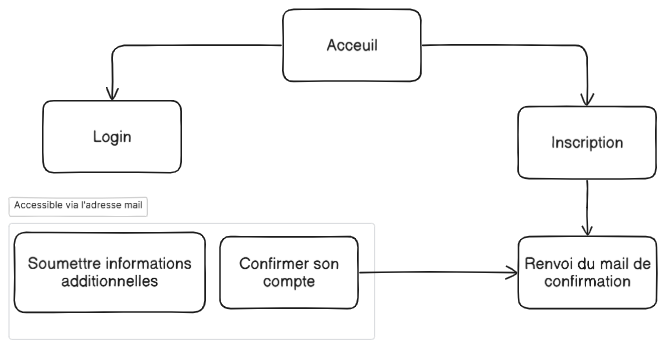
\includegraphics[width=0.6\textwidth]{images/interface/organigramme_interface_auth.png}
    \caption{Organisation de l’interface avant authentification}
    \label{fig:organigramme_non_auth}
\end{figure}

\begin{figure}[H]
    \centering
    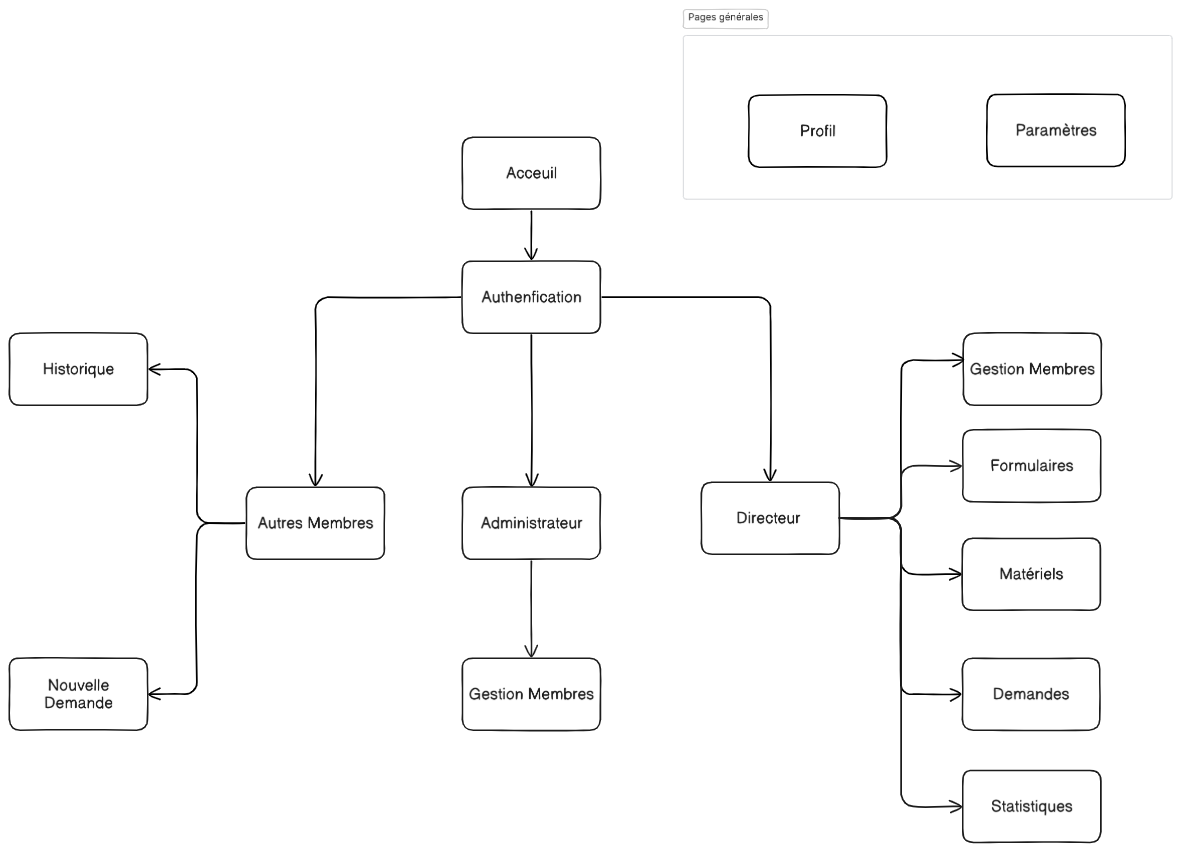
\includegraphics[width=0.9\textwidth]{images/interface/organisation_interface.png}
    \caption{Organisation de l’interface après authentification}
    \label{fig:organigramme_auth}
\end{figure}

\subsubsection{Inscription}

Cette page permet à un utilisateur de soumettre une demande d’adhésion. L'utilisateur renseigne d’abord ses informations générales, puis les détails relatifs à son rôle dans le laboratoire. Il a également la possibilité de joindre une photo de profil (optionnelle) avant de finaliser la soumission.

\begin{figure}[H]
    \centering
    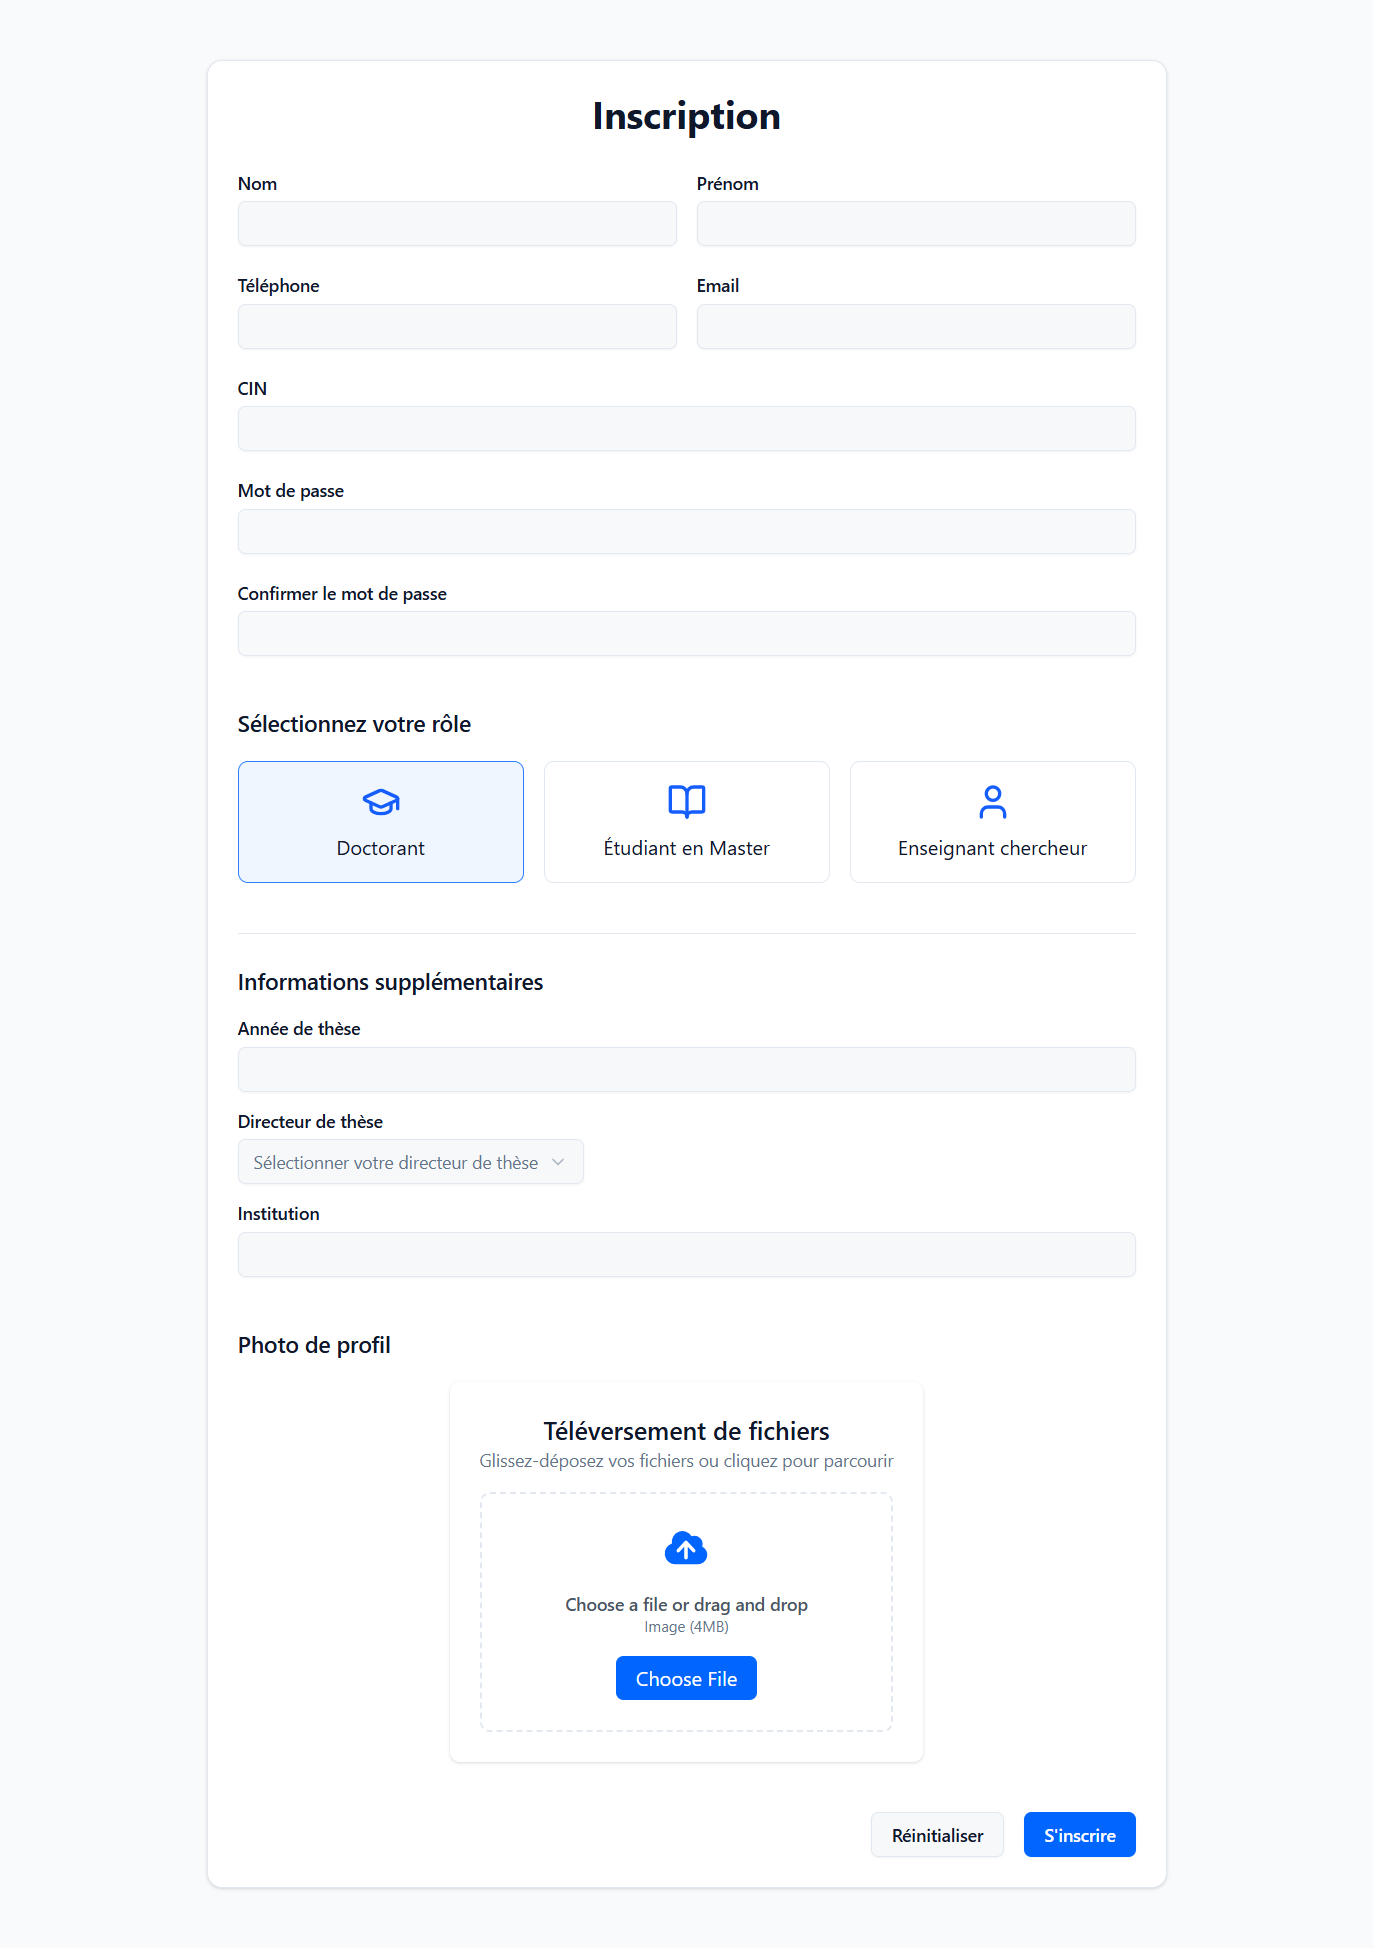
\includegraphics[width=0.5\textwidth]{images/interface/inscription.png}
    \caption{Interface d’inscription}
    \label{fig:inscription}
\end{figure}

\subsubsection{Renvoi du courriel de confirmation}

Après l’inscription, l’utilisateur peut accéder à une page dédiée au renvoi du courriel de confirmation. En cas d’expiration du jeton temporaire, il devra saisir à nouveau son adresse e-mail pour recevoir un nouveau lien de confirmation.

\begin{figure}[H]
    \centering
    
\includegraphics[width=0.6\textwidth]{images/interface/renvoie_mail.png}
    \caption{Renvoi du mail de confirmation}
    \label{fig:renvoie_mail}
\end{figure}

\begin{figure}[H]
    \centering
    
\includegraphics[width=0.6\textwidth]{images/interface/renvoie_mail_avec_mail.png}
    \caption{Renvoi du mail de confirmation avec saisie de l’adresse e-mail}
    \label{fig:renvoie_mail_avec_saisie}
\end{figure}

\subsubsection{Connexion}

La page de connexion permet à l’utilisateur d’accéder à son compte à l’aide de son adresse e-mail et de son mot de passe.

\begin{figure}[H]
    \centering
    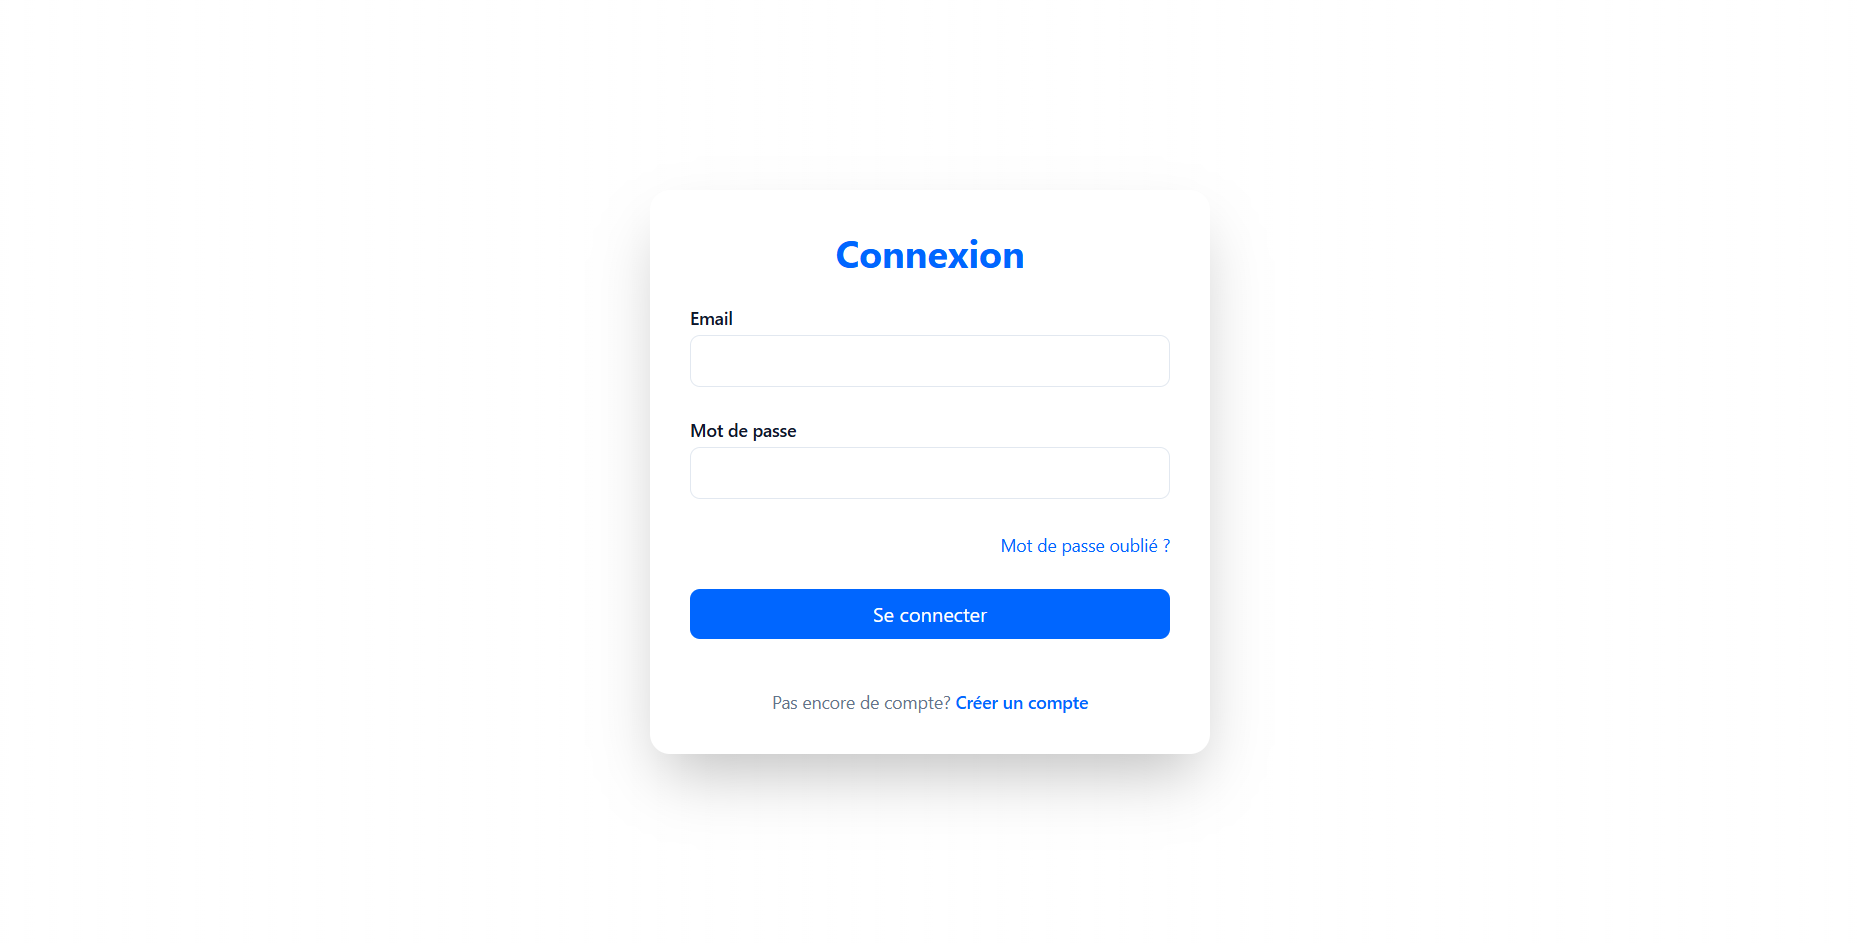
\includegraphics[width=0.7\textwidth]{images/interface/connexion.png}
    \caption{Interface de connexion}
    \label{fig:connexion}
\end{figure}

\subsubsection{Profil}

Cette section permet à l’utilisateur de consulter et de modifier les informations liées à son compte. Elle est divisée en trois parties : informations personnelles, informations académiques, et liste des étudiants encadrés (visible uniquement pour les enseignants-chercheurs et le directeur du laboratoire).

\begin{figure}[H]
    \centering
    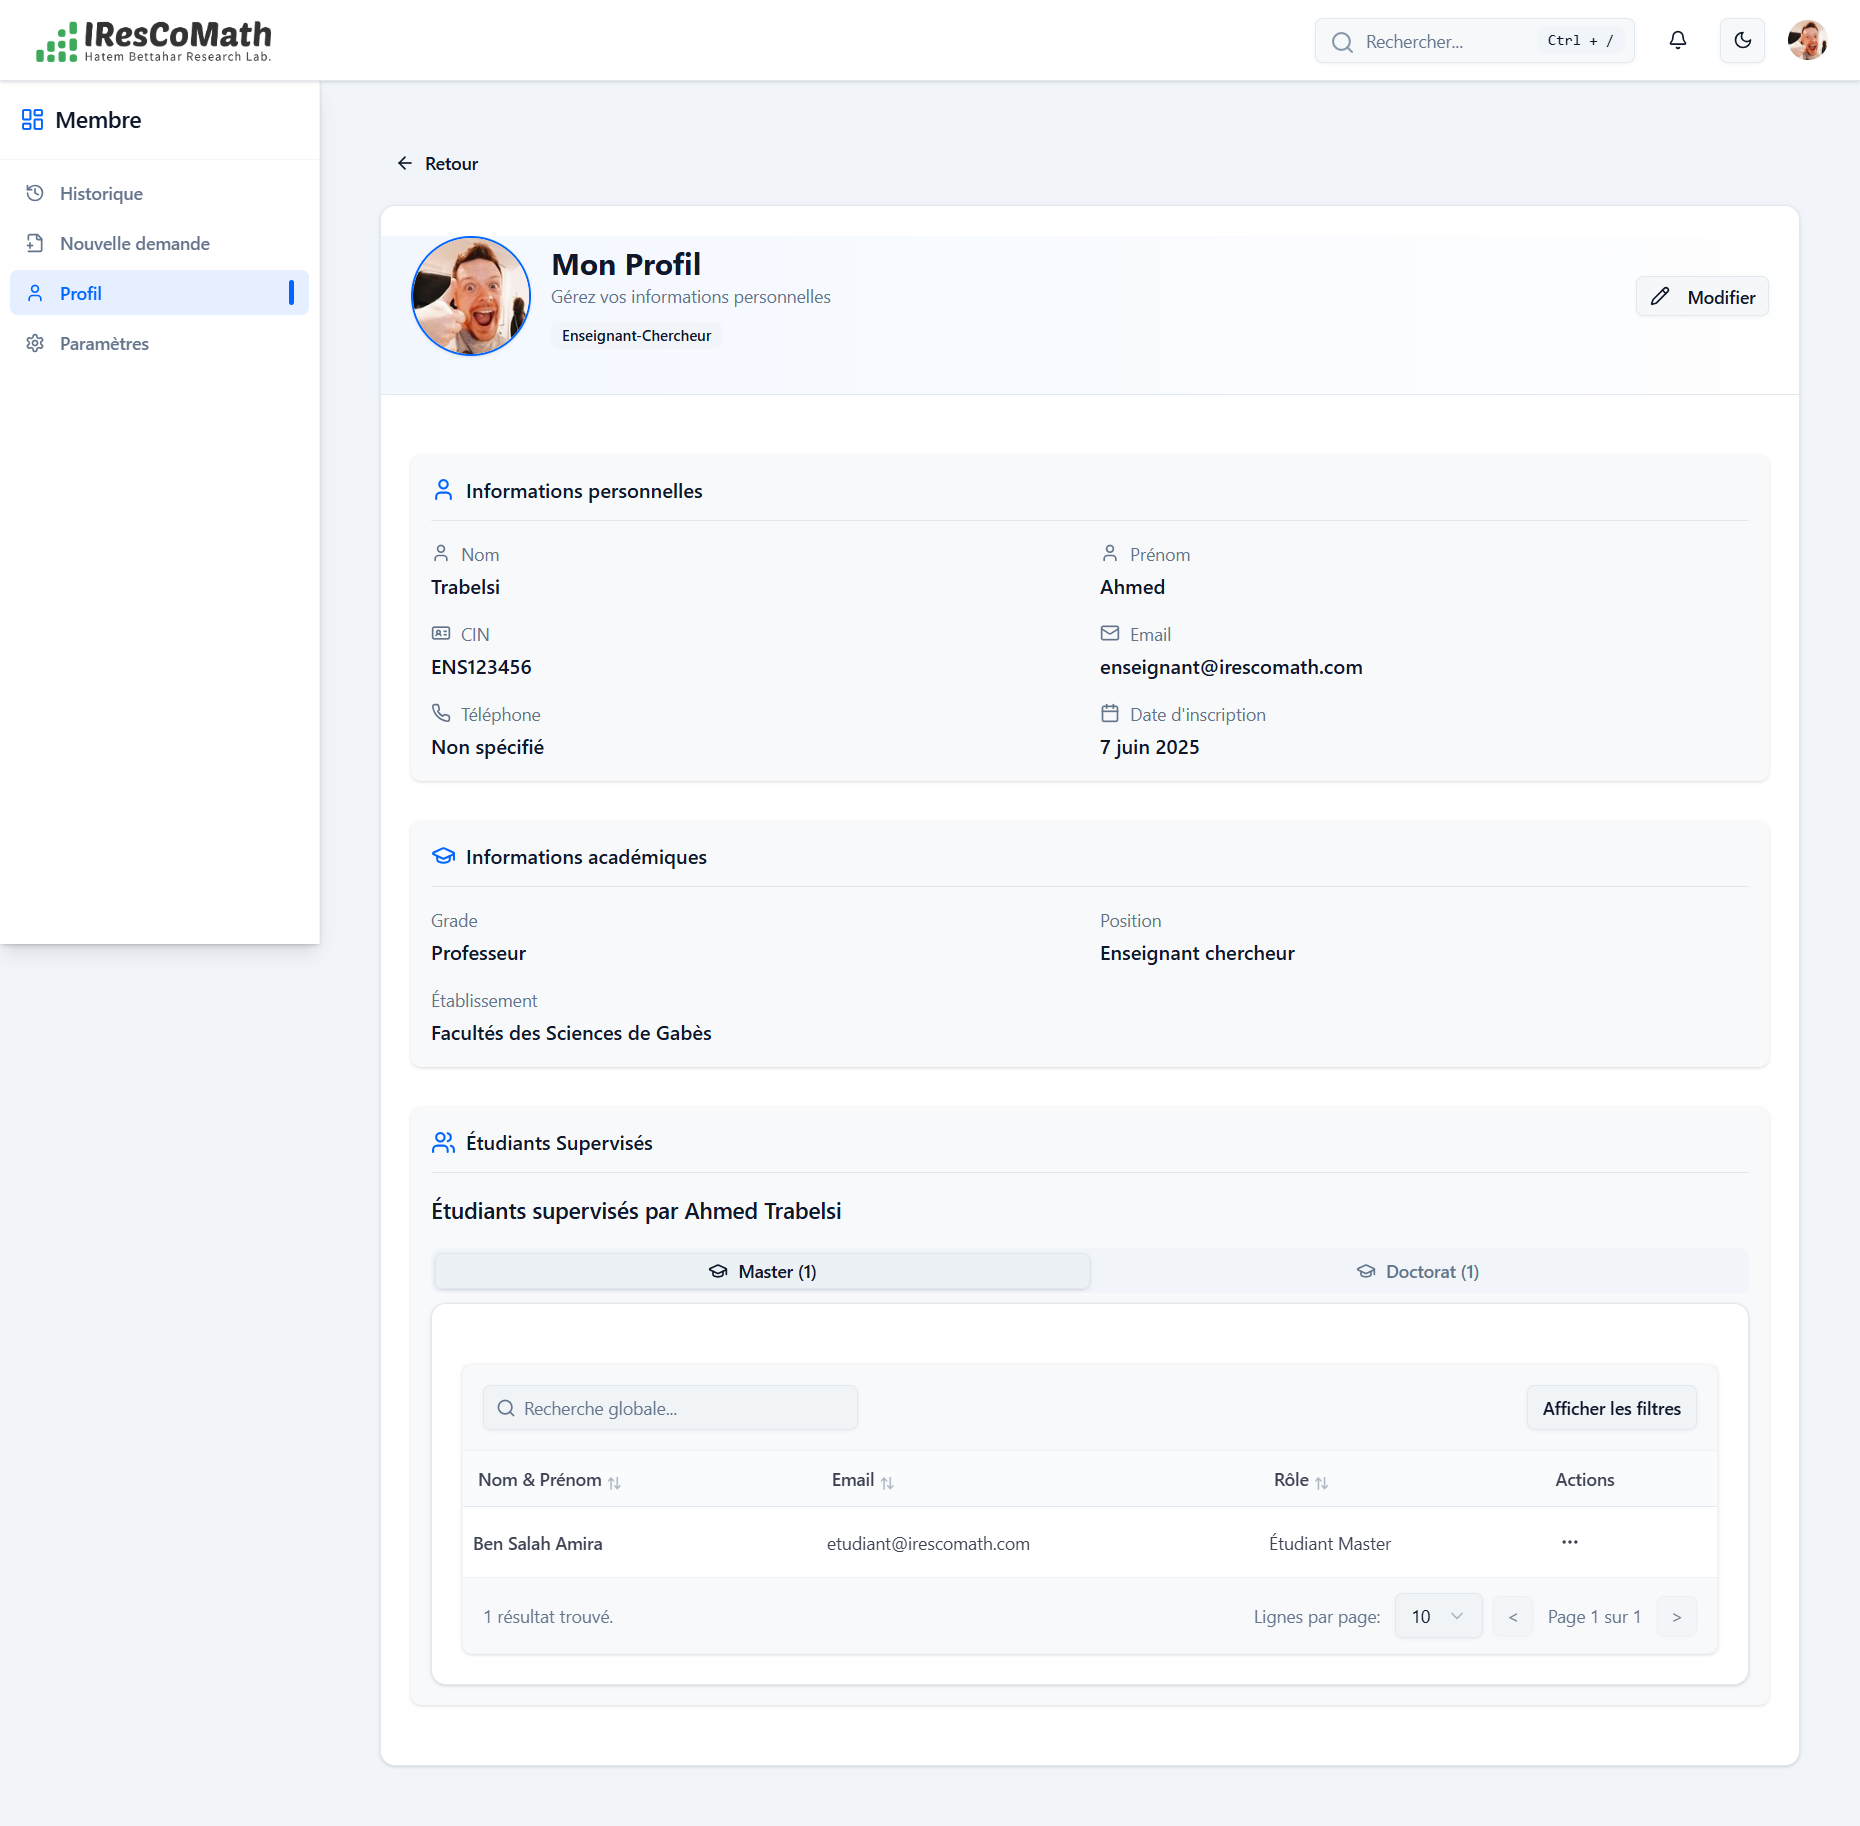
\includegraphics[width=0.7\textwidth]{images/interface/profil.png}
    \caption{Interface du profil}
    \label{fig:profil}
\end{figure}

\subsubsection{Interface du directeur de laboratoire}

Le directeur dispose d’un ensemble d’interfaces lui permettant de superviser les activités du laboratoire.

\begin{itemize}
    \item \textbf{Gestion des demandes} : tableau de bord affichant les statistiques et la liste des demandes soumises, avec possibilité de les valider, rejeter, clôturer ou consulter. Elle permet également d'accéder aux informations détaillées des demandes en cliquant sur celles-ci.
    \begin{figure}[H]
        \centering
        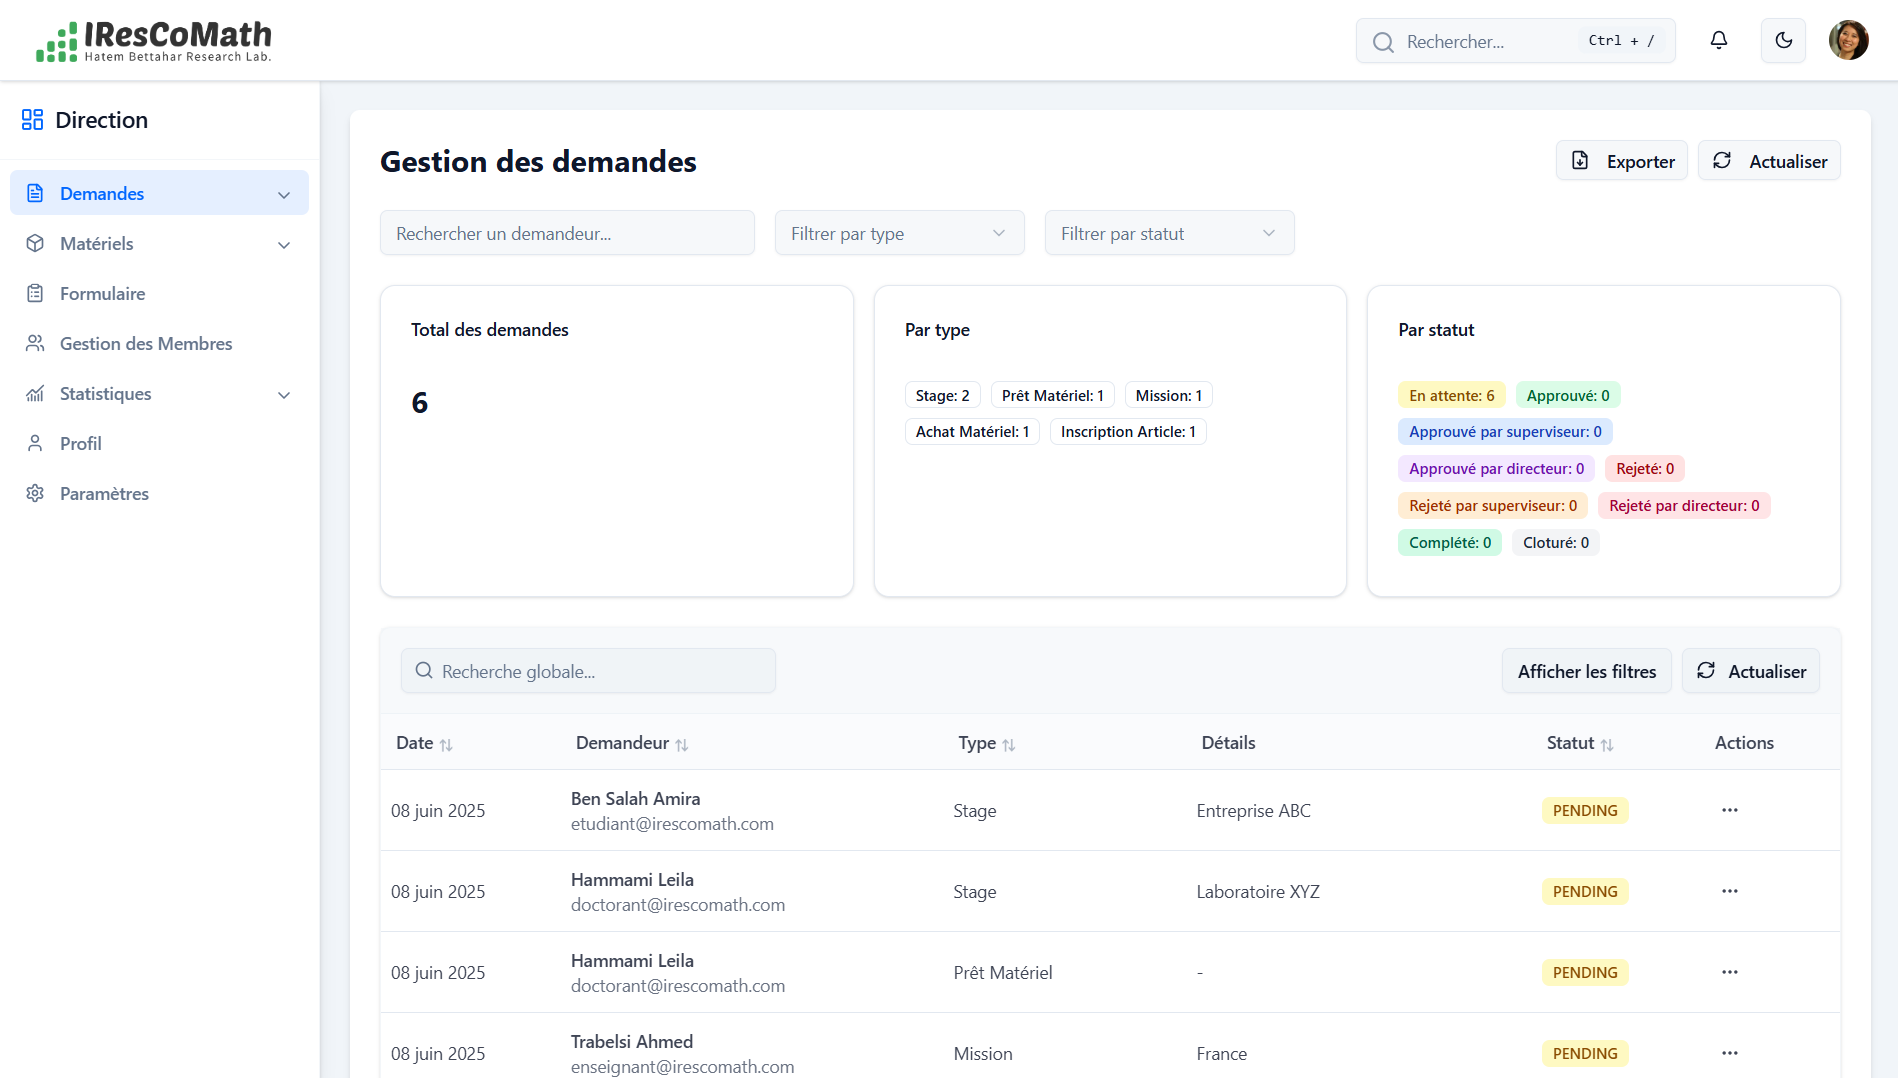
\includegraphics[width=0.7\textwidth]{images/interface/Demandes.png}
        \caption{Interface de gestion des demandes}
        \label{fig:gestion_demandes_directeur}
    \end{figure}
    \item \textbf{Gestion des matériels} : affichage, ajout, modification et suppression des matériels disponibles.
    \begin{figure}[H]
        \centering
        \includegraphics[width=0.7\textwidth]{images/interface/materiels.png}
        \caption{Interface de gestion des matériels}
        \label{fig:gestion_materiels_directeur}
    \end{figure}

    \item \textbf{Gestion des formulaires} : gestion des modèles de formulaires à travers les opérations classiques (ajout, édition, suppression).
    \begin{figure}[H]
        \centering
        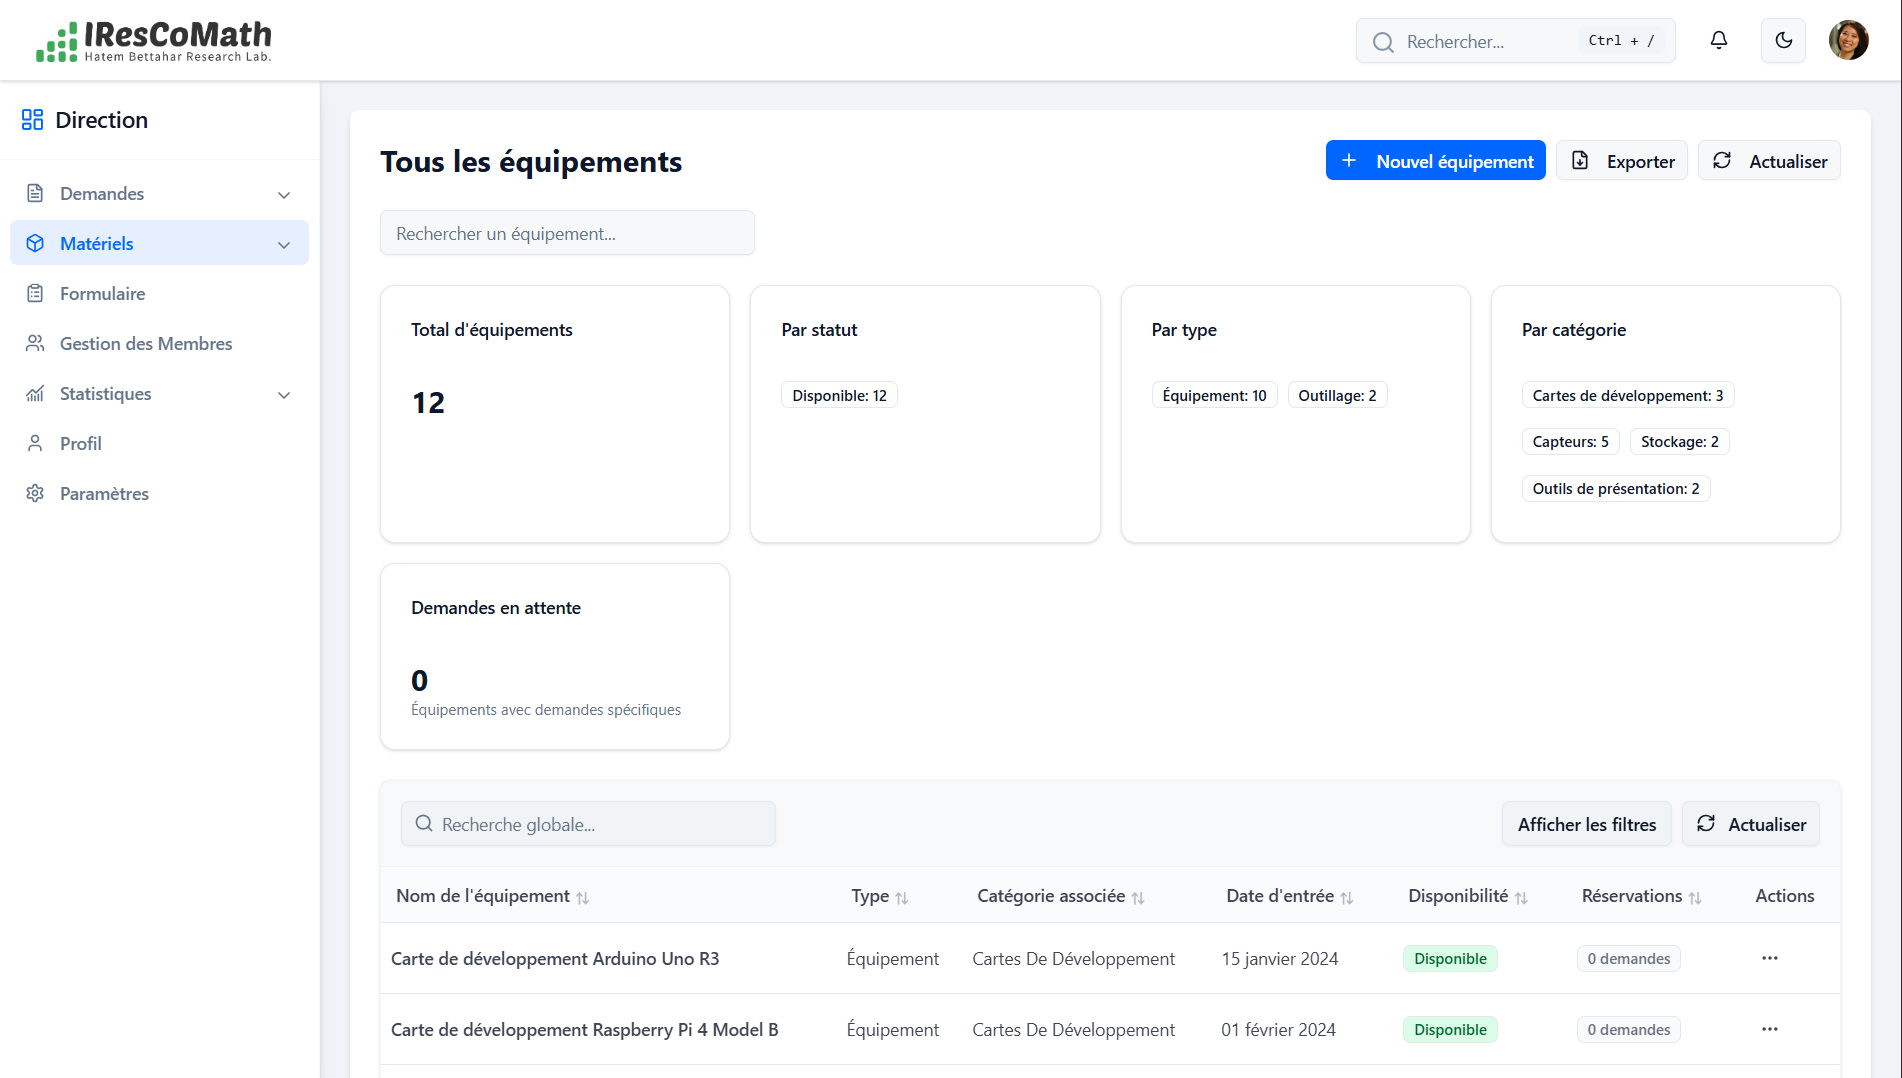
\includegraphics[width=0.7\textwidth]{images/interface/Formulaires.png}
        \caption{Interface de gestion des formulaires}
        \label{fig:gestion_formulaires_directeur}
    \end{figure}

    \item \textbf{Gestion des membres} : consultation des membres inscrits et des demandes d’adhésion. Possibilité de valider ou de rejeter une demande.
    \begin{figure}[H]
        \centering
        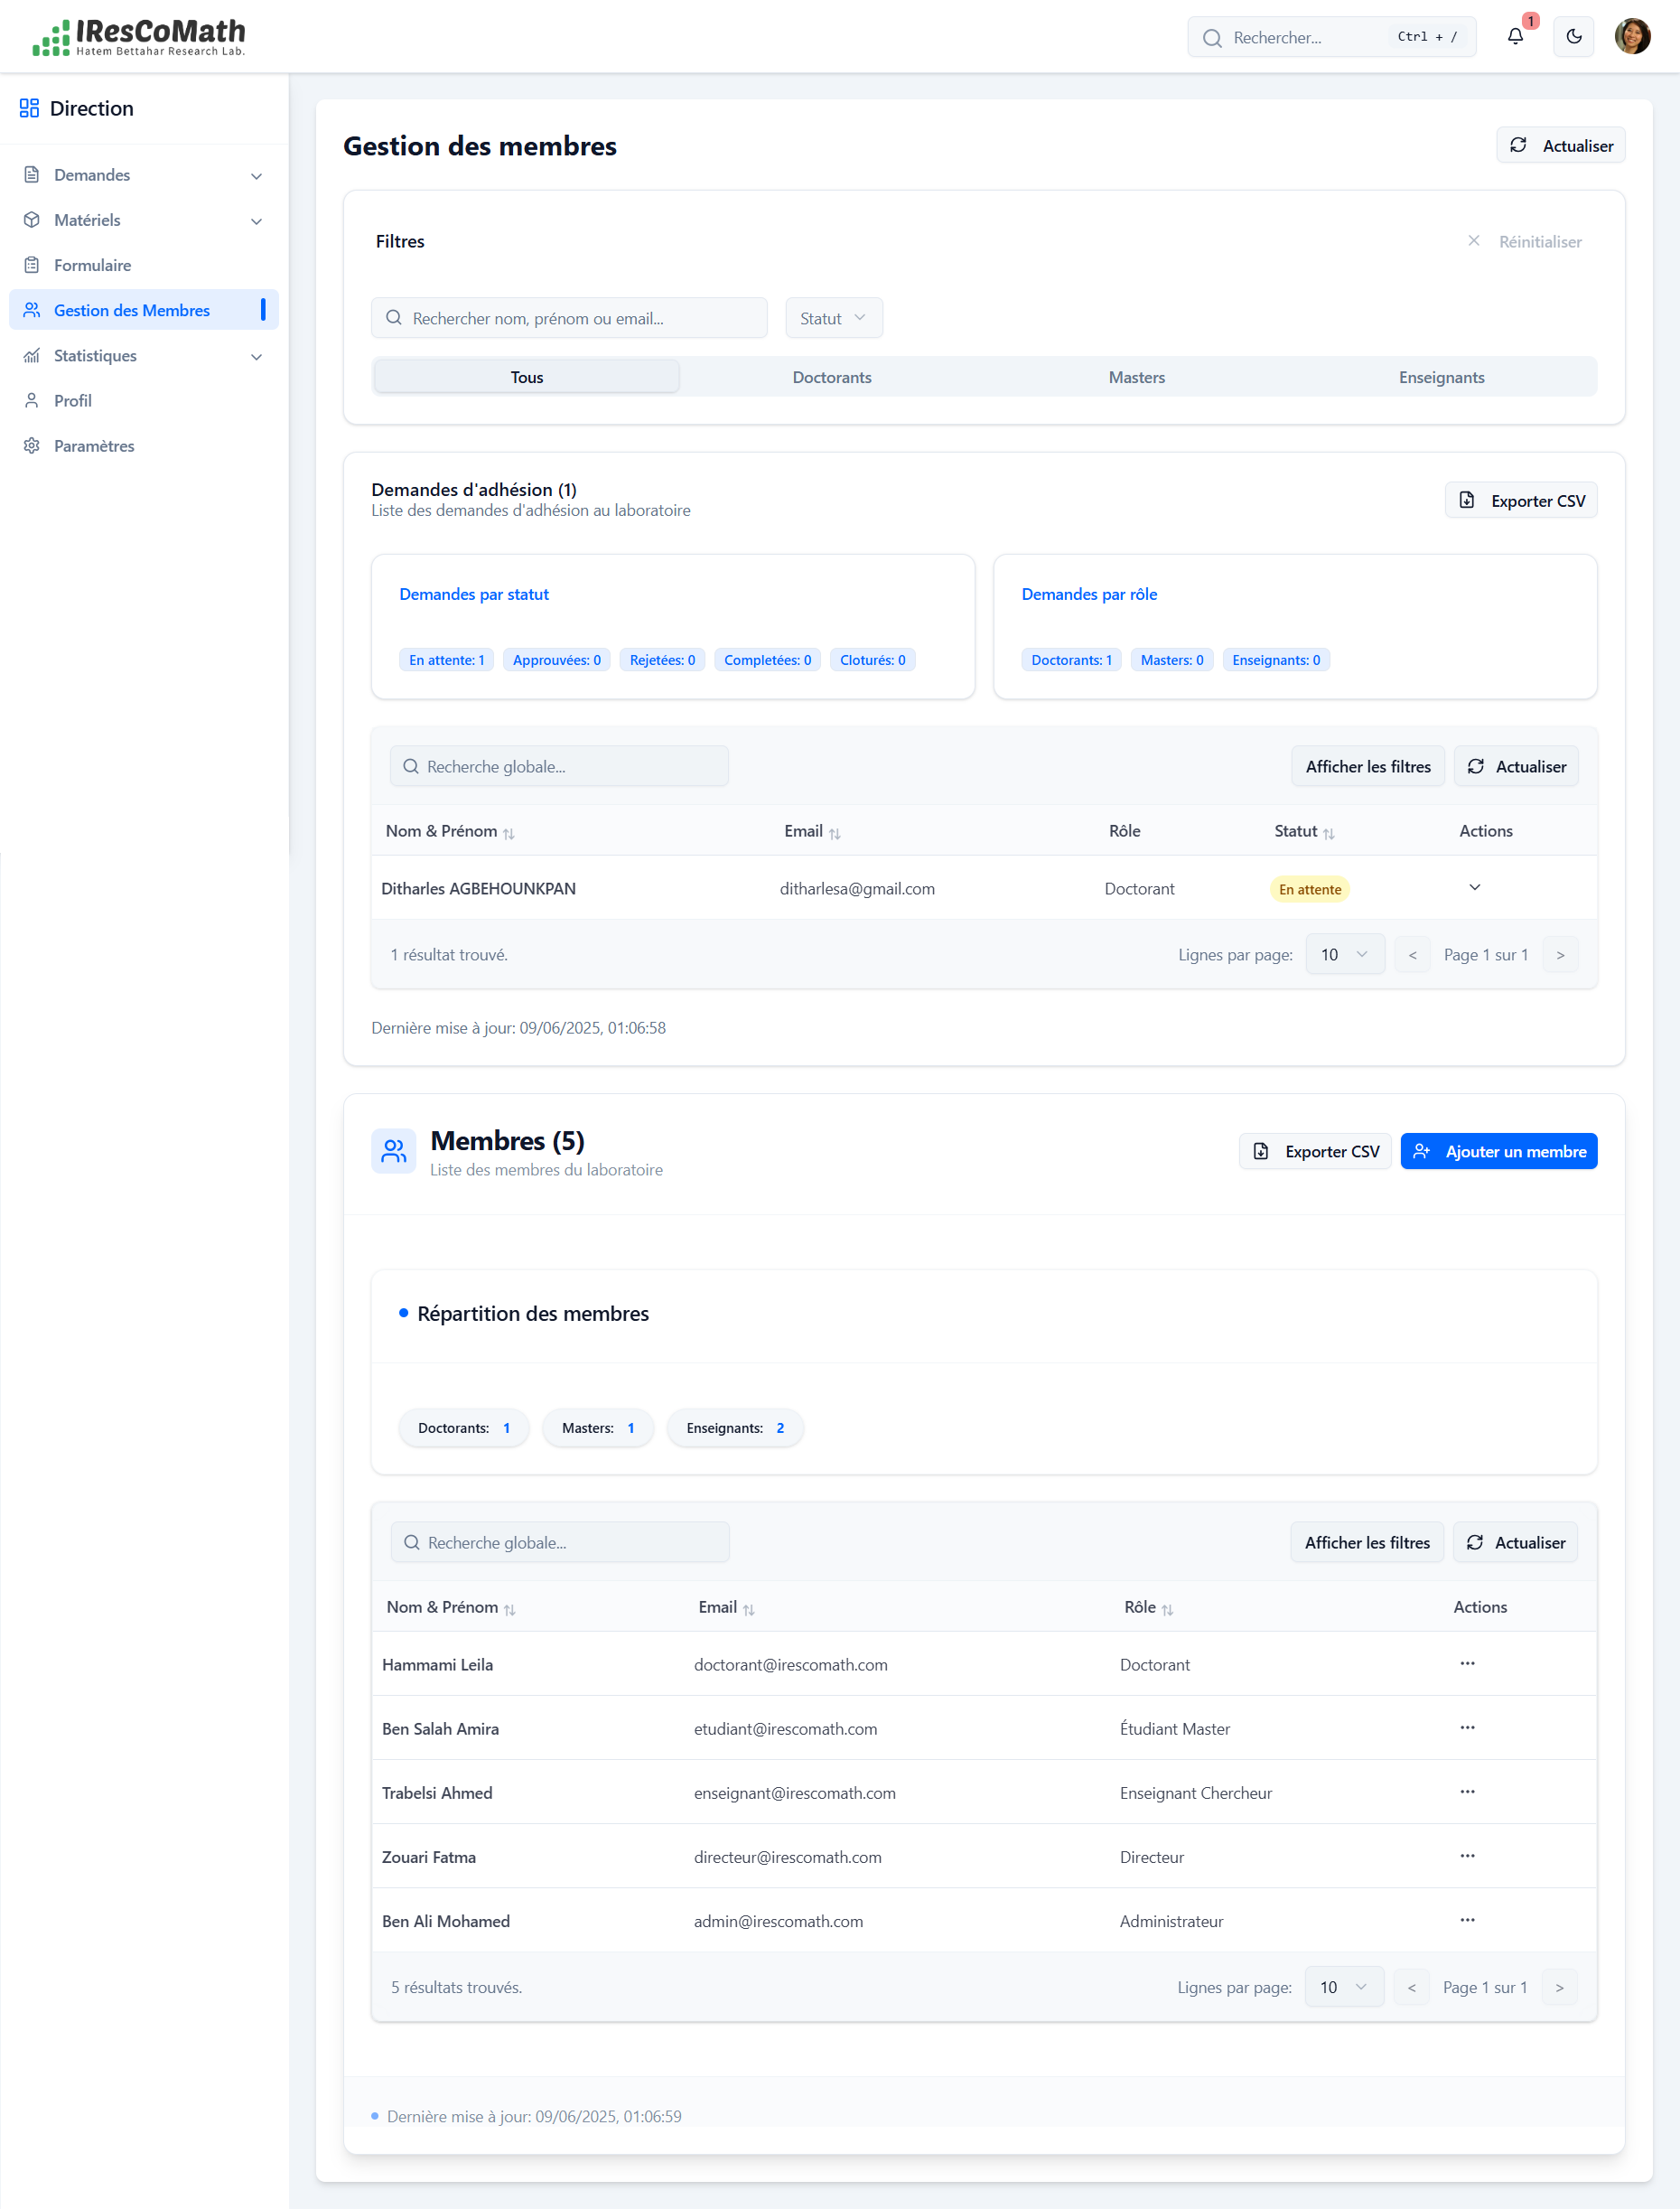
\includegraphics[width=0.62\textwidth]{images/interface/Membres.png}
        \caption{Interface de gestion des membres}
        \label{fig:gestion_membres_directeur}
    \end{figure}

    \item \textbf{Statistiques globales} : graphiques et statistiques globales sur les entités du système (demandes, matériels,  membres).
    \begin{figure}[H]
        \centering
        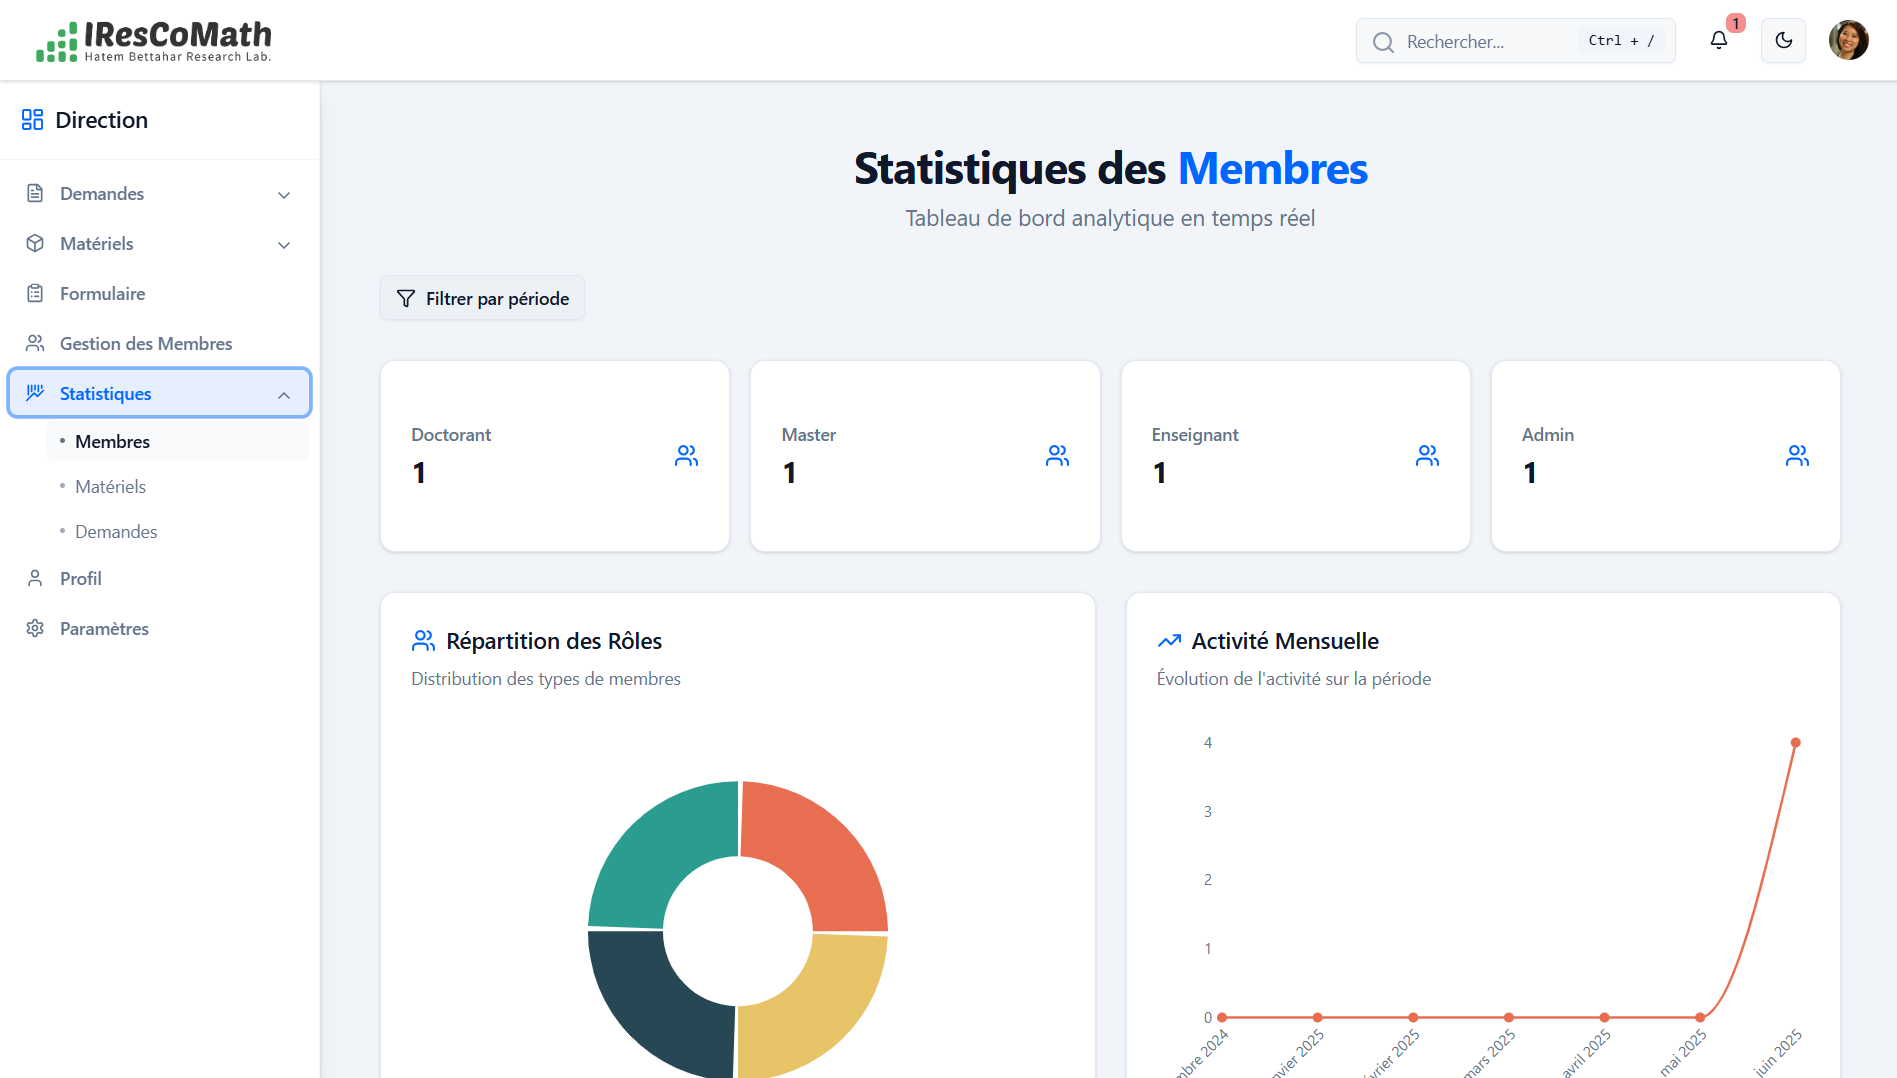
\includegraphics[width=0.7\textwidth]{images/interface/Statistiques.png}
        \caption{Interface des statistiques}
        \label{fig:statistiques}
    \end{figure}
\end{itemize}
En plus des pages mentionnées précédemment, le directeur du laboratoire a également accès aux pages suivantes : \textbf{l’ajout et la modification des matériels}, \textbf{l’ajout et la modification des catégories de matériels}, \textbf{l’ajout et la modification des formulaires}, ainsi que \textbf{les pages détaillant les informations d’un membre, d’une demande, d’un matériel, d’un formulaire ou d’un équipement}.

\subsubsection{Interface des membres du laboratoire}

Les membres du laboratoire (étudiants, enseignants-chercheurs, etc.) disposent également de plusieurs interfaces :

\begin{itemize}
    \item \textbf{Gestion de leurs propres demandes} : cette interface, similaire à celle de l’administrateur, affiche uniquement les demandes créées par le membre. Il peut les consulter, les modifier, les supprimer, ou les compléter.
  
    \item \textbf{Soumission de nouvelles demandes} : selon son rôle, un membre peut accéder à différents types de formulaires. Par exemple, un enseignant-chercheur peut soumettre une demande de participation à un article scientifique.
    \begin{figure}[H]
        \centering
        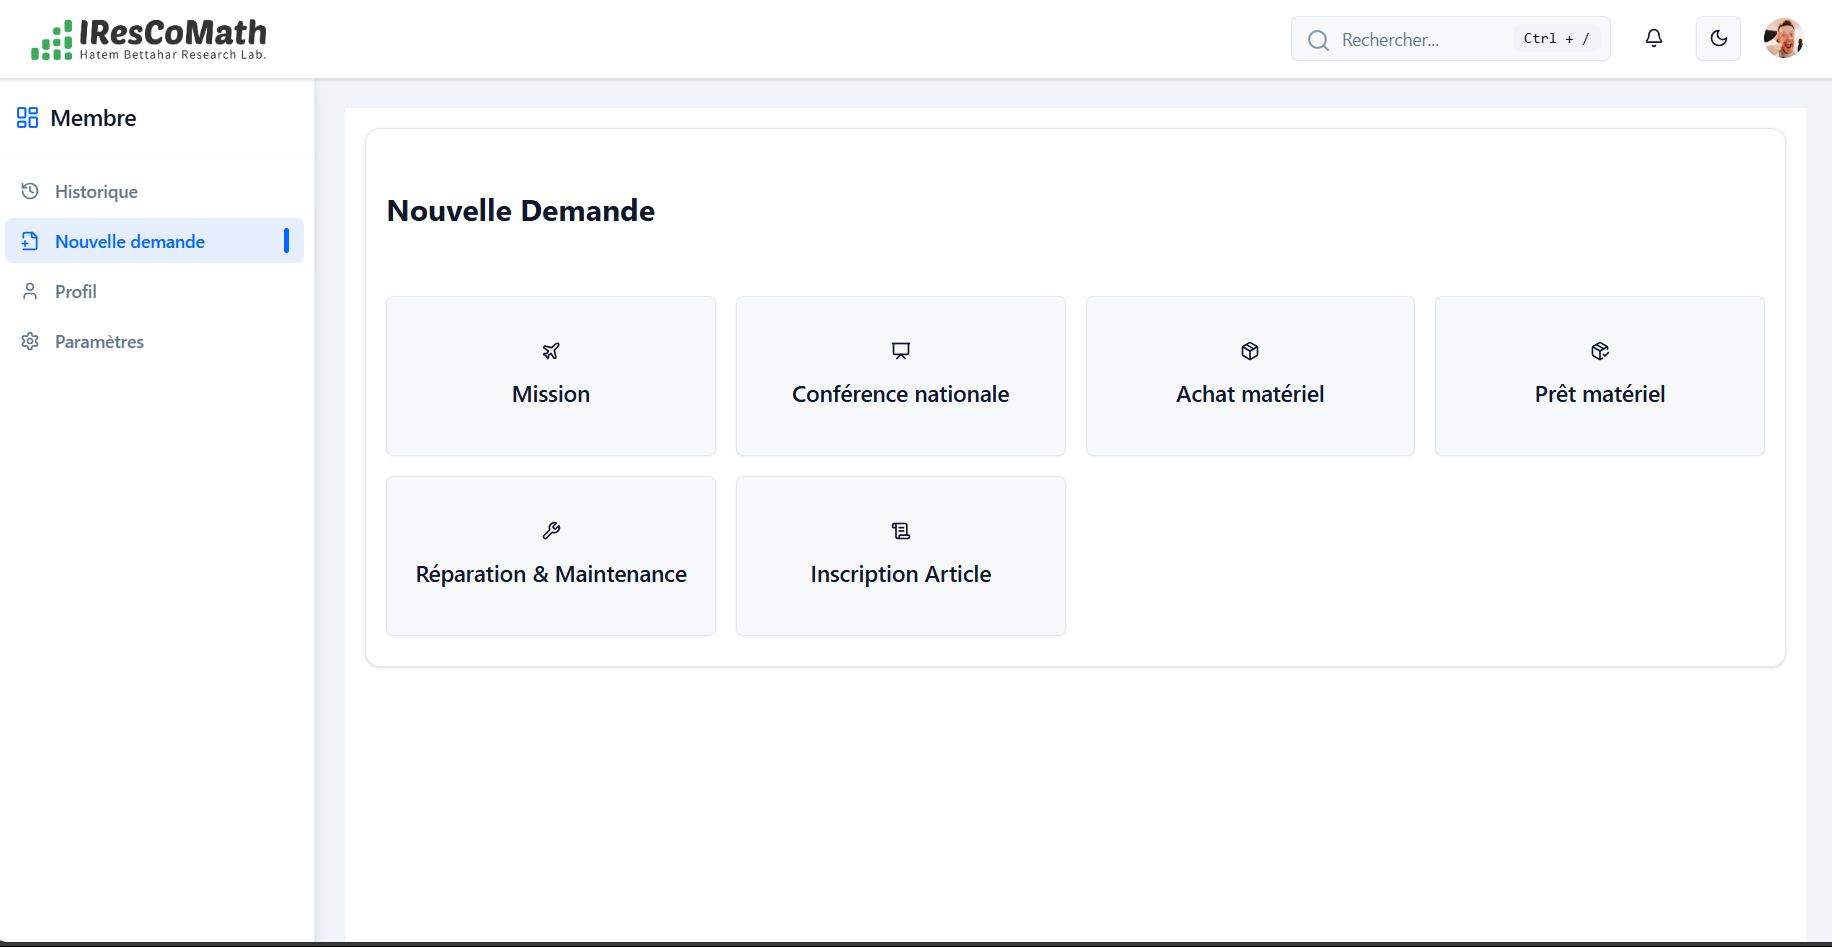
\includegraphics[width=0.7\textwidth]{images/interface/nouvelle_demande.png}
        \caption{Interface de soumission de nouvelles demandes}
        \label{fig:nouvelles_demandes}
    \end{figure}

    \begin{figure}[H]
        \centering
        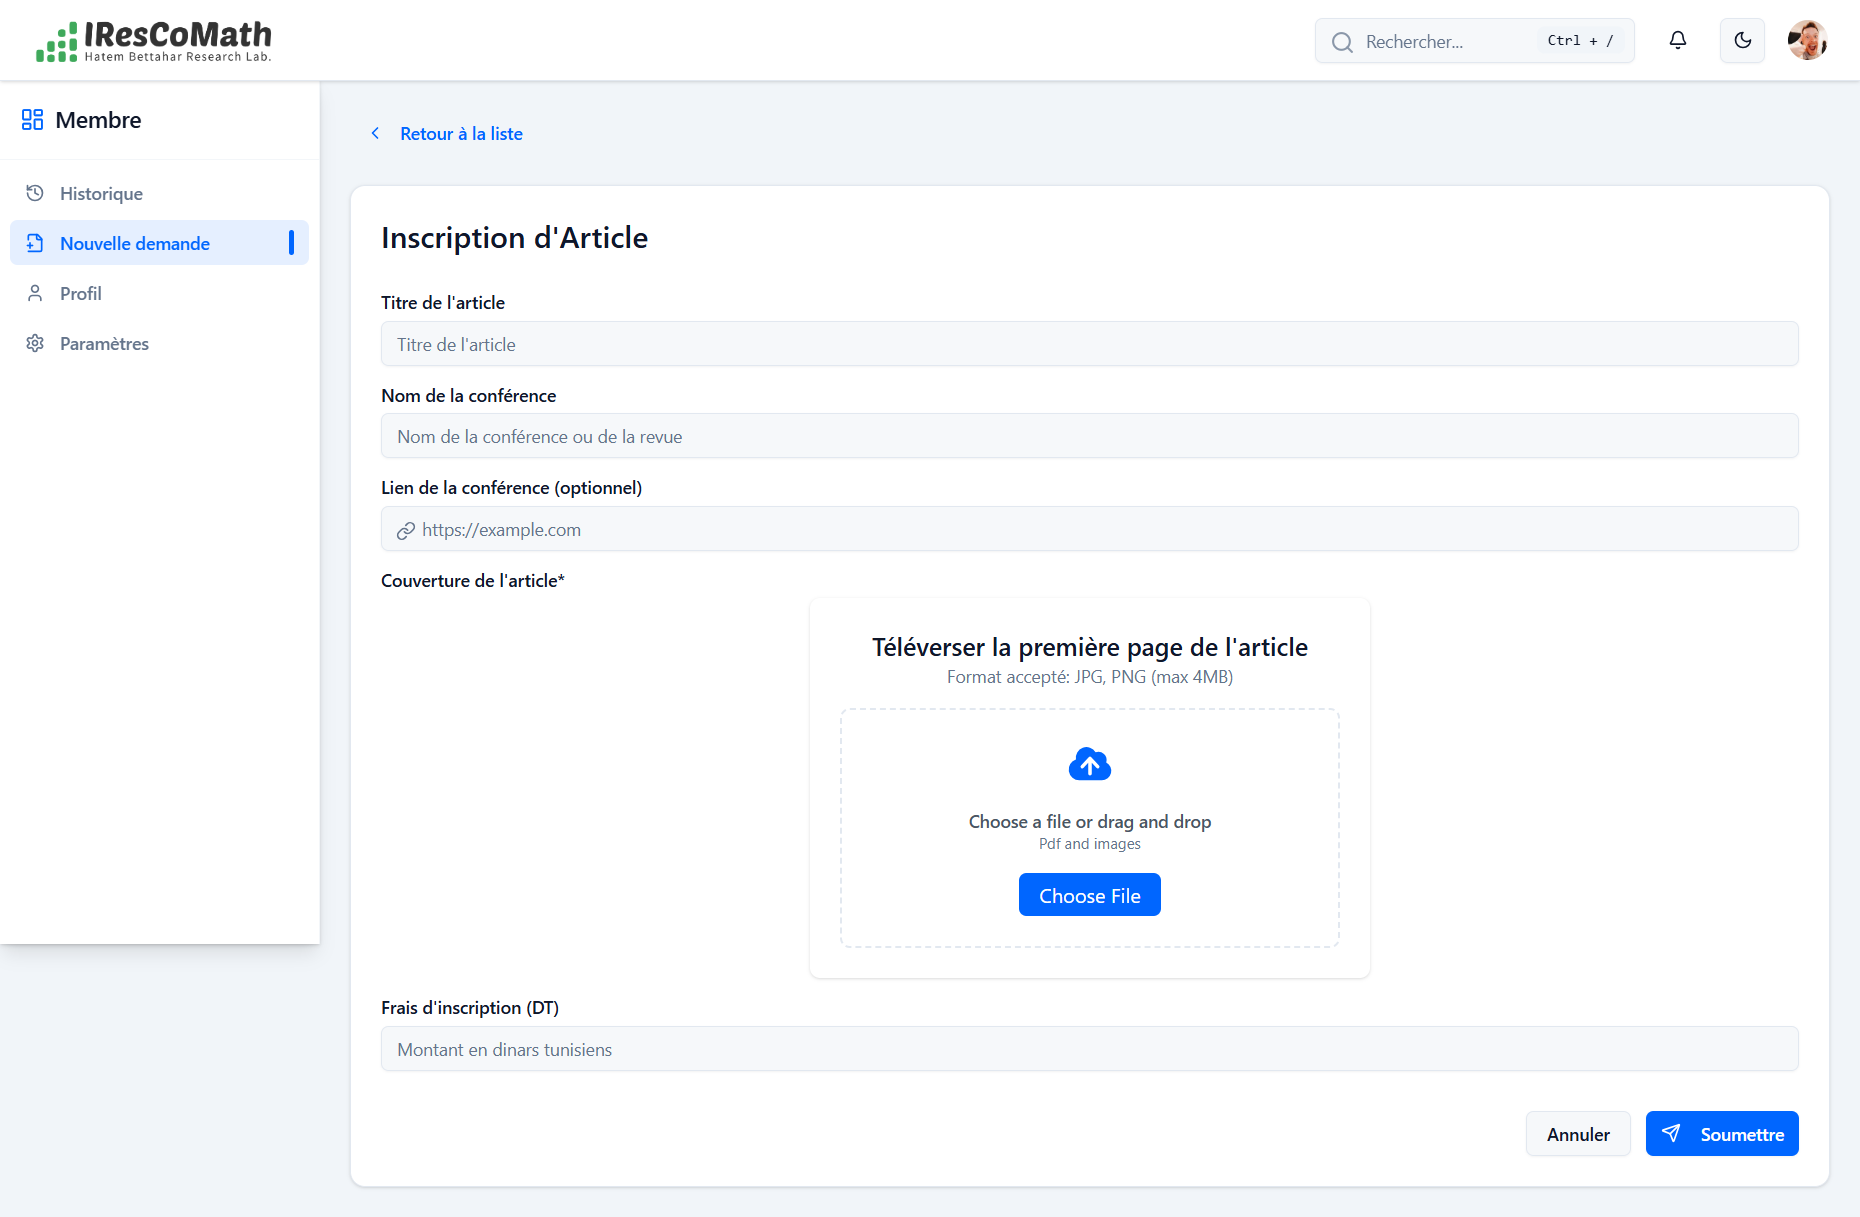
\includegraphics[width=0.7\textwidth]{images/interface/inscriptionArticle.png}
        \caption{Formulaire de soumission d’un article scientifique}
        \label{fig:articleScientifique}
    \end{figure}
\end{itemize}
\subsection{Backend}
\subsubsection{Architecture générale}

Le backend a été développé avec pour objectif principal de maintenir une architecture modulaire et évolutive, répondant aux exigences de développement, de maintenabilité et de sécurité. Il est conçu sous forme d'une API RESTful. L’architecture s’organise en plusieurs couches distinctes :

\begin{itemize}
  \item \textbf{routes} : Ce dossier définit les différentes routes de l'API ainsi que les méthodes HTTP associées ;
  \item \textbf{controllers} : Contient les fonctions de traitement des requêtes, la validation des données entrantes et la gestion des réponses ;
  \item \textbf{services} : Regroupe la logique métier et les interactions complexes avec la base de données ;
  \item \textbf{prisma} : Contient la configuration et la connexion à la base de données via l’ORM Prisma ;
  \item \textbf{middlewares} : Comporte des fonctions exécutées avant ou après les requêtes (authentification, autorisation, gestion des erreurs, etc.) ;
  \item \textbf{utils} : Réunit des fonctions utilitaires communes à plusieurs modules de l’application ;
  \item \textbf{constants} : Contient des constantes globales utilisées dans l’ensemble du projet ;
  \item \textbf{types} : Définit des types TypeScript partagés dans l'application.
\end{itemize}

Cette organisation modulaire permet de séparer clairement les responsabilités, facilitant ainsi la maintenance, les tests et l'évolution du système. De plus, l’utilisation de Prisma simplifie la gestion des données relationnelles grâce à une abstraction efficace. La figure suivante illustre la communication entre les différents composants du backend :

\begin{figure}[H]
  \centering
  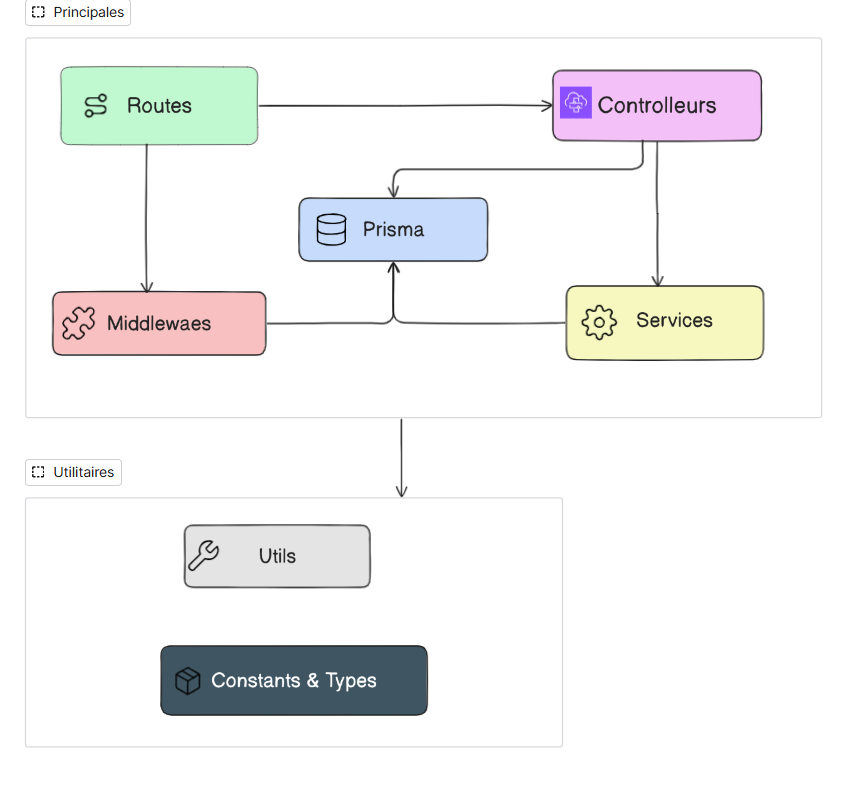
\includegraphics[width=0.9\textwidth]{images/backend/file.png}
  \caption{Schéma de communication entre les composants du backend}
  \label{fig:communication_backend}
\end{figure}

\subsubsection{Couches métier et logique applicative}

\paragraph{Routes et endpoints de l’API} Les routes de l'API sont organisées en sept groupes principaux :

\begin{itemize}
  \item \textbf{auth} : Authentification et autorisation des utilisateurs ;
  \item \textbf{validate} : Gestion des demandes d’adhésion ;
  \item \textbf{users} : Gestion des utilisateurs et de leurs profils ;
  \item \textbf{requests} : Création, modification et suivi des demandes diverses ;
  \item \textbf{equipments} : Gestion du matériel (ajout, suppression, mise à jour) ;
  \item \textbf{notifications} : Envoi et gestion des notifications système ;
  \item \textbf{templates} : Gestion dynamique des modèles de formulaires.
\end{itemize}

\paragraph{Services et controllers}  
Les services et les contrôleurs sont organisés de manière modulaire et suivent la logique des routes. À chaque route correspond un contrôleur responsable de la gestion des requêtes entrantes, de la validation des données et de la réponse. Les services encapsulent la logique métier et interagissent avec la base de données. Cette séparation permet une meilleure testabilité et une évolutivité facilitée.

\paragraph{Middlewares}

Les middlewares sont des fonctions intermédiaires exécutées avant ou après le traitement des requêtes. Dans notre application, deux middlewares principaux sont utilisés :

\begin{itemize}
  \item \textbf{verifyToken} : Vérifie la validité du token JWT et l’authentification de l’utilisateur ;
  \item \textbf{checkRole} : Vérifie les rôles et les droits d’accès de l’utilisateur.
\end{itemize}

\subsubsection{Journalisation et surveillance}

Afin d'assurer un suivi efficace des activités de l'application et de faciliter le débogage, un système de journalisation a été mis en place à l'aide de la bibliothèque \textbf{Pino}. Il s'agit d'un logger rapide et performant pour Node.js, compatible avec la production.

\begin{itemize}
  \item \textbf{Performance} : Pino est optimisé pour minimiser l'impact sur les performances grâce à une sérialisation JSON ultra-rapide.
  \item \textbf{Lisibilité et structuration} : Les logs sont structurés, horodatés et peuvent être enrichis avec des métadonnées utiles (utilisateur, route, niveau de gravité, etc.).
  \item \textbf{Niveaux de log} : L’application utilise différents niveaux de log (info, warn, error, debug) pour catégoriser les événements selon leur importance.
  \item \textbf{Intégration} : Pino est intégré aux middlewares pour journaliser automatiquement les requêtes HTTP entrantes, les réponses, ainsi que les erreurs serveur.
\end{itemize}

Grâce à cette journalisation structurée, il est plus simple d’identifier les anomalies, de retracer les actions effectuées par les utilisateurs, et de surveiller le comportement global de l’application.

\subsubsection{Gestion des données et infrastructure}

\paragraph{Prisma et PostgreSQL}

L’ORM Prisma offre une abstraction puissante et typée pour interagir avec la base de données.Le choix de Prisma s’explique par sa capacité à générer un client typé, ce qui permet une meilleure sécurité au moment du développement, et réduit les erreurs liées aux requêtes SQL. De plus, il s’intègre naturellement à TypeScript et facilite la migration de la base de donnée. Ce choix favorise la productivité des développeurs tout en réduisant les risques d'erreurs comme les injections SQL. La base de données PostgreSQL a été choisie pour ses performances, sa robustesse et sa forte compatibilité avec les modèles relationnels complexes.

\paragraph{Uploadthing}

Pour la gestion des fichiers, nous avons opté pour Uploadthing, une solution moderne et sécurisée d’hébergement de fichiers. Elle permet une intégration fluide avec les applications JavaScript/TypeScript, tout en garantissant la sécurité et la fiabilité de l’upload et du stockage. Cette solution a été choisie pour sa documentation complète, sa flexibilité et sa facilité de mise en œuvre.

\section{Tests et validation}
\subsection{Stratégie de test}
Une approche de test en boîte noire a été adoptée, centrée sur la vérification du comportement attendu de chaque fonctionnalité.

\subsection{Tests de sécurité}



\begin{itemize}
  \item \textbf{Tests d’authentification} : Vérification de la gestion des sessions utilisateurs ;
  \item \textbf{Tests d’autorisation} : Contrôle des permissions en fonction des rôles ;
  \item \textbf{Tests de validation des données} : Protection contre les injections et les entrées malveillantes ;
  \item \textbf{Tests de gestion des tokens} : Sécurité du JWT et gestion de leur expiration.
\end{itemize}

\subsection{Tests utilisateurs}

Des tests ont été menés auprès de plusieurs profils (étudiants, enseignants, administrateurs) afin d’évaluer l’ergonomie, la compréhension de l’interface et l'efficacité des parcours utilisateurs. Ces retours ont permis d'apporter plusieurs ajustements à l’interface et à l’expérience utilisateur.

\subsection{Tests automatisés}

Des tests automatisés unitaires et d’intégration ont été mis en place pour certaines fonctionnalités critiques, dans une optique de fiabilité, de régression minimale et de maintenance évolutive.

\subsection{Tests fonctionnels}

\begin{itemize}
  \item \textbf{Tests de création de demandes} : Vérification de la validation des formulaires et des contraintes métier ;
  \item \textbf{Tests de workflow} : Contrôle du routage des demandes selon les profils utilisateurs ;
  \item \textbf{Tests de notification} : Vérification des alertes et notifications automatiques ;
  \item \textbf{Tests de gestion des fichiers} : Téléversement, stockage et récupération des fichiers.
\end{itemize}

\subsection{Tests d’interface utilisateur}

\begin{itemize}
  \item \textbf{Tests de navigation} : Vérification de la cohérence des parcours utilisateurs ;
  \item \textbf{Tests de responsivité} : Adaptation de l’interface sur différentes tailles d’écran ;
  
  \item \textbf{Tests multi-navigateurs} : Compatibilité avec les navigateurs modernes (Chrome, Firefox, Safari).
\end{itemize}

\section{Déploiement}

L'application a été développée et testée en environnement local, puis déployée en production sur la plateforme cloud Railway. Ce choix permet un déploiement rapide et continu, tout en assurant une haute disponibilité et une gestion simplifiée de l'infrastructure.

\begin{figure}[H]
    \centering
    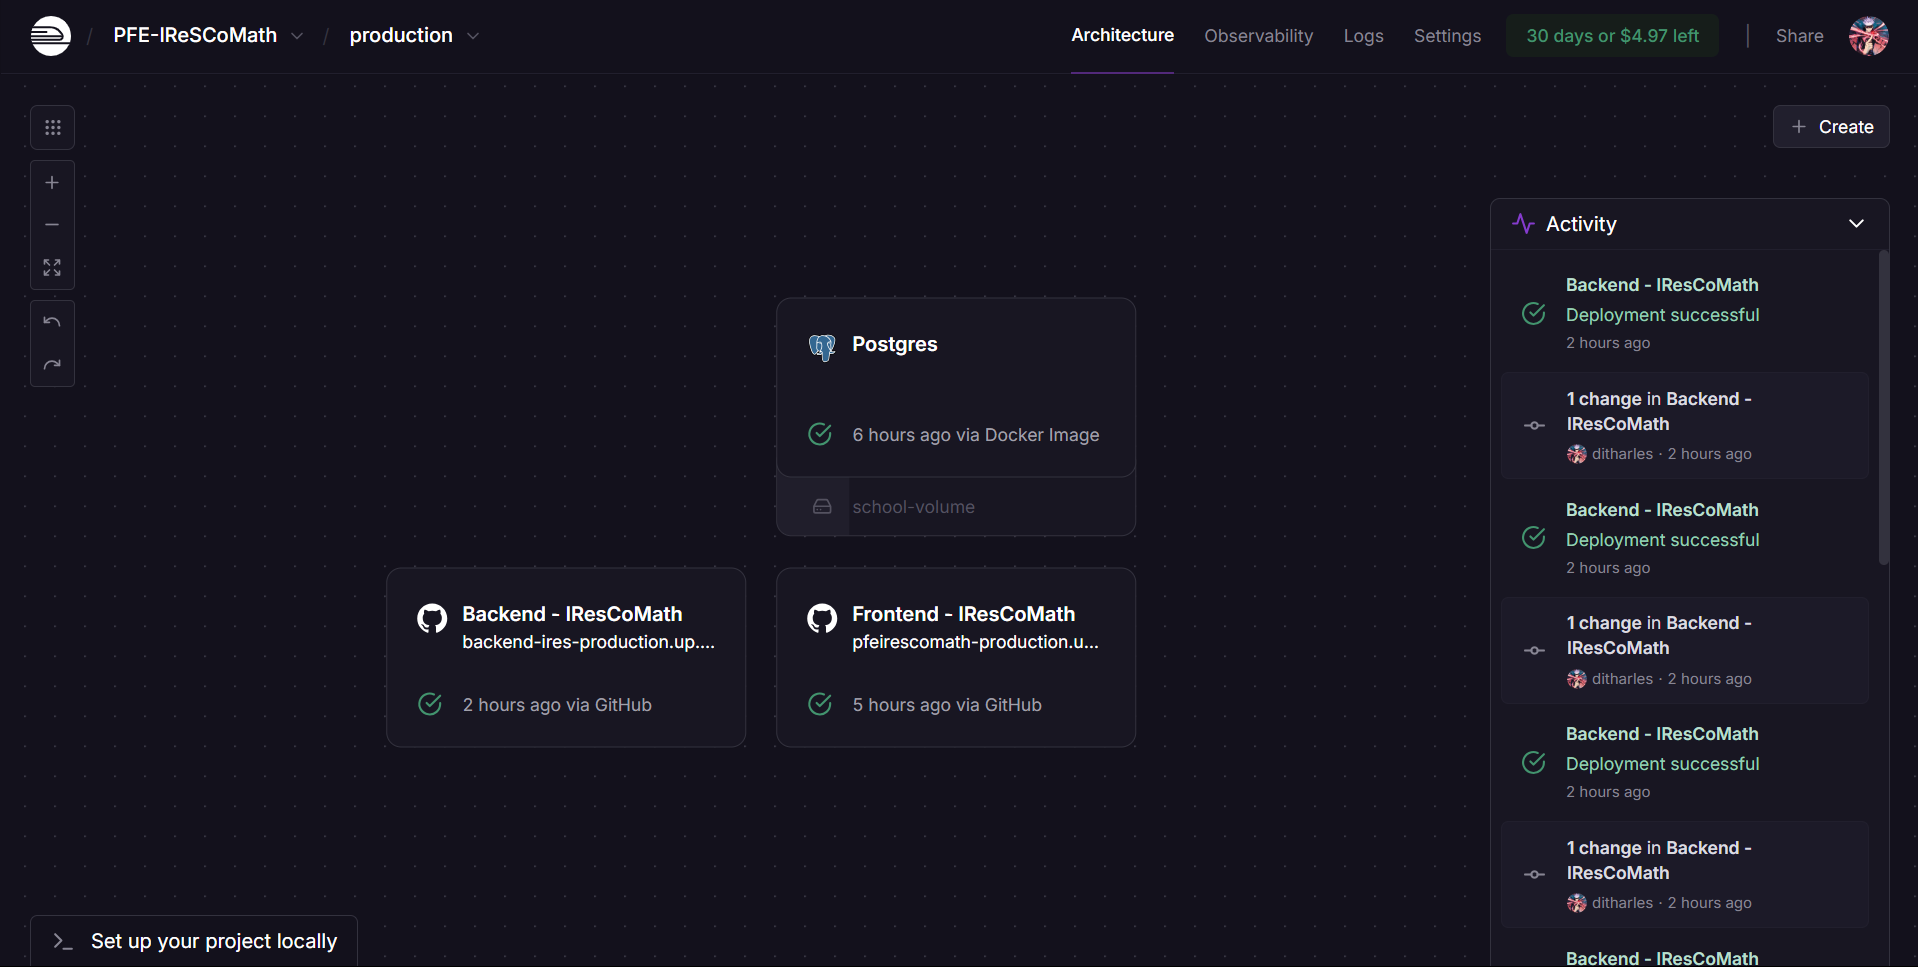
\includegraphics[width=0.7\textwidth]{images/backend/deploiement.png}
    \caption{Déploiement sur Railway}
    \label{fig:deploiement}
\end{figure}

\section{Conclusion}

Ce chapitre a présenté la mise en œuvre technique du projet, en détaillant l’architecture backend, l’organisation du code, les stratégies de test, ainsi que le déploiement en production. Grâce à une architecture modulaire, une gestion efficace des données et une série de tests rigoureux, l’application offre robustesse, évolutivité et sécurité. Le chapitre suivant présentera les résultats obtenus et les perspectives d’amélioration envisagées.
